\chapter{Analyse des données}

 Les données fournies contiennent des informations sur les causes de décès et la population en Angleterre et au Pays de Galles entre 1979 et 1992, sous la forme de tables. Nous allons tout d'abord analyser ces tables, afin d'en comprendre le contenu et d'en vérifier la validité. Pour celà, nous avons effectuer plusieurs requêtes SQL par table, en vérifiant par exemple l'unicité des clés, la logique des chiffres obtenus, en comparant nos résultats à des sources officielles, l'unicité des districts par county... Nous avons de plus effectuer des requêtes de visualisation des données, pour voir par exemple la répartition des décès par sexe pour chaque cause ( On a donc découvert que, surprise !, il n'y a pas de décès ayant pour cause un avortement, chez le sexe masculin).\\


\begin{paragraph}
Les données sont formées de 19 tables, liées entre elles par des clés étrangères. Nous avons tout d'abord remarqué que les données des deux premières années (79 et 80) sont des estimations (chiffres ronds et calculs justes). En effet, les données étaient manquantes pour ces deux années, et elles ont été estimées par rapport aux évolutions des autres années. Commençons tout d'abord par les tables concernant la population. La table principale est "7992pops", et compte 214 396 lignes. Elle contient le nombre de personnes vivantes, dans les régions citées précédemment, en fonction de l'année, du district, de l'age et du sexe. Ces différentes informations (sauf l'année) sont en fait des identifiants, à mettre en relation avec d'autre tables. Nous avons vérifier, grâce à une requête SQL, que la clé de cette table était bien composé des identifiants de county, district, sexage et de l'année.\\
Les identifiants de county et de district peuvent donner le nom du district concerné, dans la table "cdlist". Il existe 403 districts, contenus dans des county, eux-même contenus dans des régions. \\
Ils permettent aussi de faire le lien avec la table "areaclas", qui contient elle aussi pour chaque paire d'identifiants le nom du district, ainsi que les codes et noms des familles, groupes et clusters. Ceux-ci sont des classifications des districts selon des critères économiques. \\
A partir de l'identifiant du county, on peut retrouver son nom et l'identifiant de la région à laquelle il appartient grâce à la table "county". Il existe 54 county.\\
De la même façon, à partir de l'identifiant de la région, on peut faire le lien avec la table "region", qui permet de retrouver son nom (il y en a 11 en tout). \\
On peut ensuite retrouver l'âge et le sexe de la catégorie à partir de l'identifiant sexage, que l'on retrouve dans la table "sexage". Cette table contient les identifiants associés à des labels, ceux-ci étant de la forme M1-4 ou encore W5-9, représentant respectivement des garçons agés de 1 à 4 ans, et des filles agées de 5 à 9 ans. Ce découpage permet de classer la population selon 38 catégories de sexage.\\
\end{paragraph}

\begin{paragraph}
Nous allons maintenant nous intéresser aux données concernant les morts. Ces données étant vraiment très imposantes, elles sont séparées en 11 tables, une par région : "yorkhumb", "westmids", "stheast", "wales", "sthwest", "nthwest", "london", "ntheast", mersey", "eastmids" et "eastern". De même que précédement, les différentes lignes correspondent au nombre de morts selon l'année, le disctrict, la catégorie sexage, avec en plus la cause. \\
La cause est en fait un identifiant correspondant à une ligne de la table "causes". Chaque cause a un nom, un niveau et un père. Elles sont réparties selon un arbre de causes : la cause 1 correspond à la cause "toutes les causes", cette cause a des fils qui elles-mêmes ont des fils, et plus le niveau est élevé, plus la cause de mort est précise. Le père de la cause correspond donc à son père dans l'arbre. Normalement, toutes les morts de causes de niveau 1 devraient être égales à toutes les morts de cause de niveau 2 ainsi que toutes les sommes sur les niveau. En réalité, grâce des requêtes SQL adéquates, nous avons réalisé que les sommes n'étaient pas égales. Ceci est probablement du à des erreurs ou des oublis lors du remplissage des certificats. Il existe aussi une autre cause, renseignée dans le document fourni (\textbf{``local mortaility datapack.pdf''})~: Un nouveau certificat pour les morts néonatales a été introduit en 1986, et ces morts ne sont plus rentrées sous la cause ``Certain conditions originating in the perinatal period'' depuis cette date là.\\
\end{paragraph}

\begin{paragraph}
Il reste maintenant le fichier sample.csv, qui contient les données concernant les morts de néoplasies pour le comté de Bedfordshire uniquement. Après l'avoir importé en tant que table dans la base de données, nous avons pu l'analyser. Il est semblable aux tables de morts par région : elle contient le nombre de morts pour une catégorie de sexage, une année et une cause. Nous nous sommes rendu compte que pour cette table, les causes n'étaient pas considérées de la même façon. En effet, contrairement aux autres morts, celles-ci ne sont comptées qu'une fois, à leur niveau de cause le plus précis. On peut ensuite remonter aux causes plus générales à l'aide de la relation père-fils de ces causes.
\end{paragraph}

\pagebreak


\chapter{Modélisation de l'entrepôt et des cubes}

\section{Hypercube Population}
\begin{figure}[h]
    \centering
    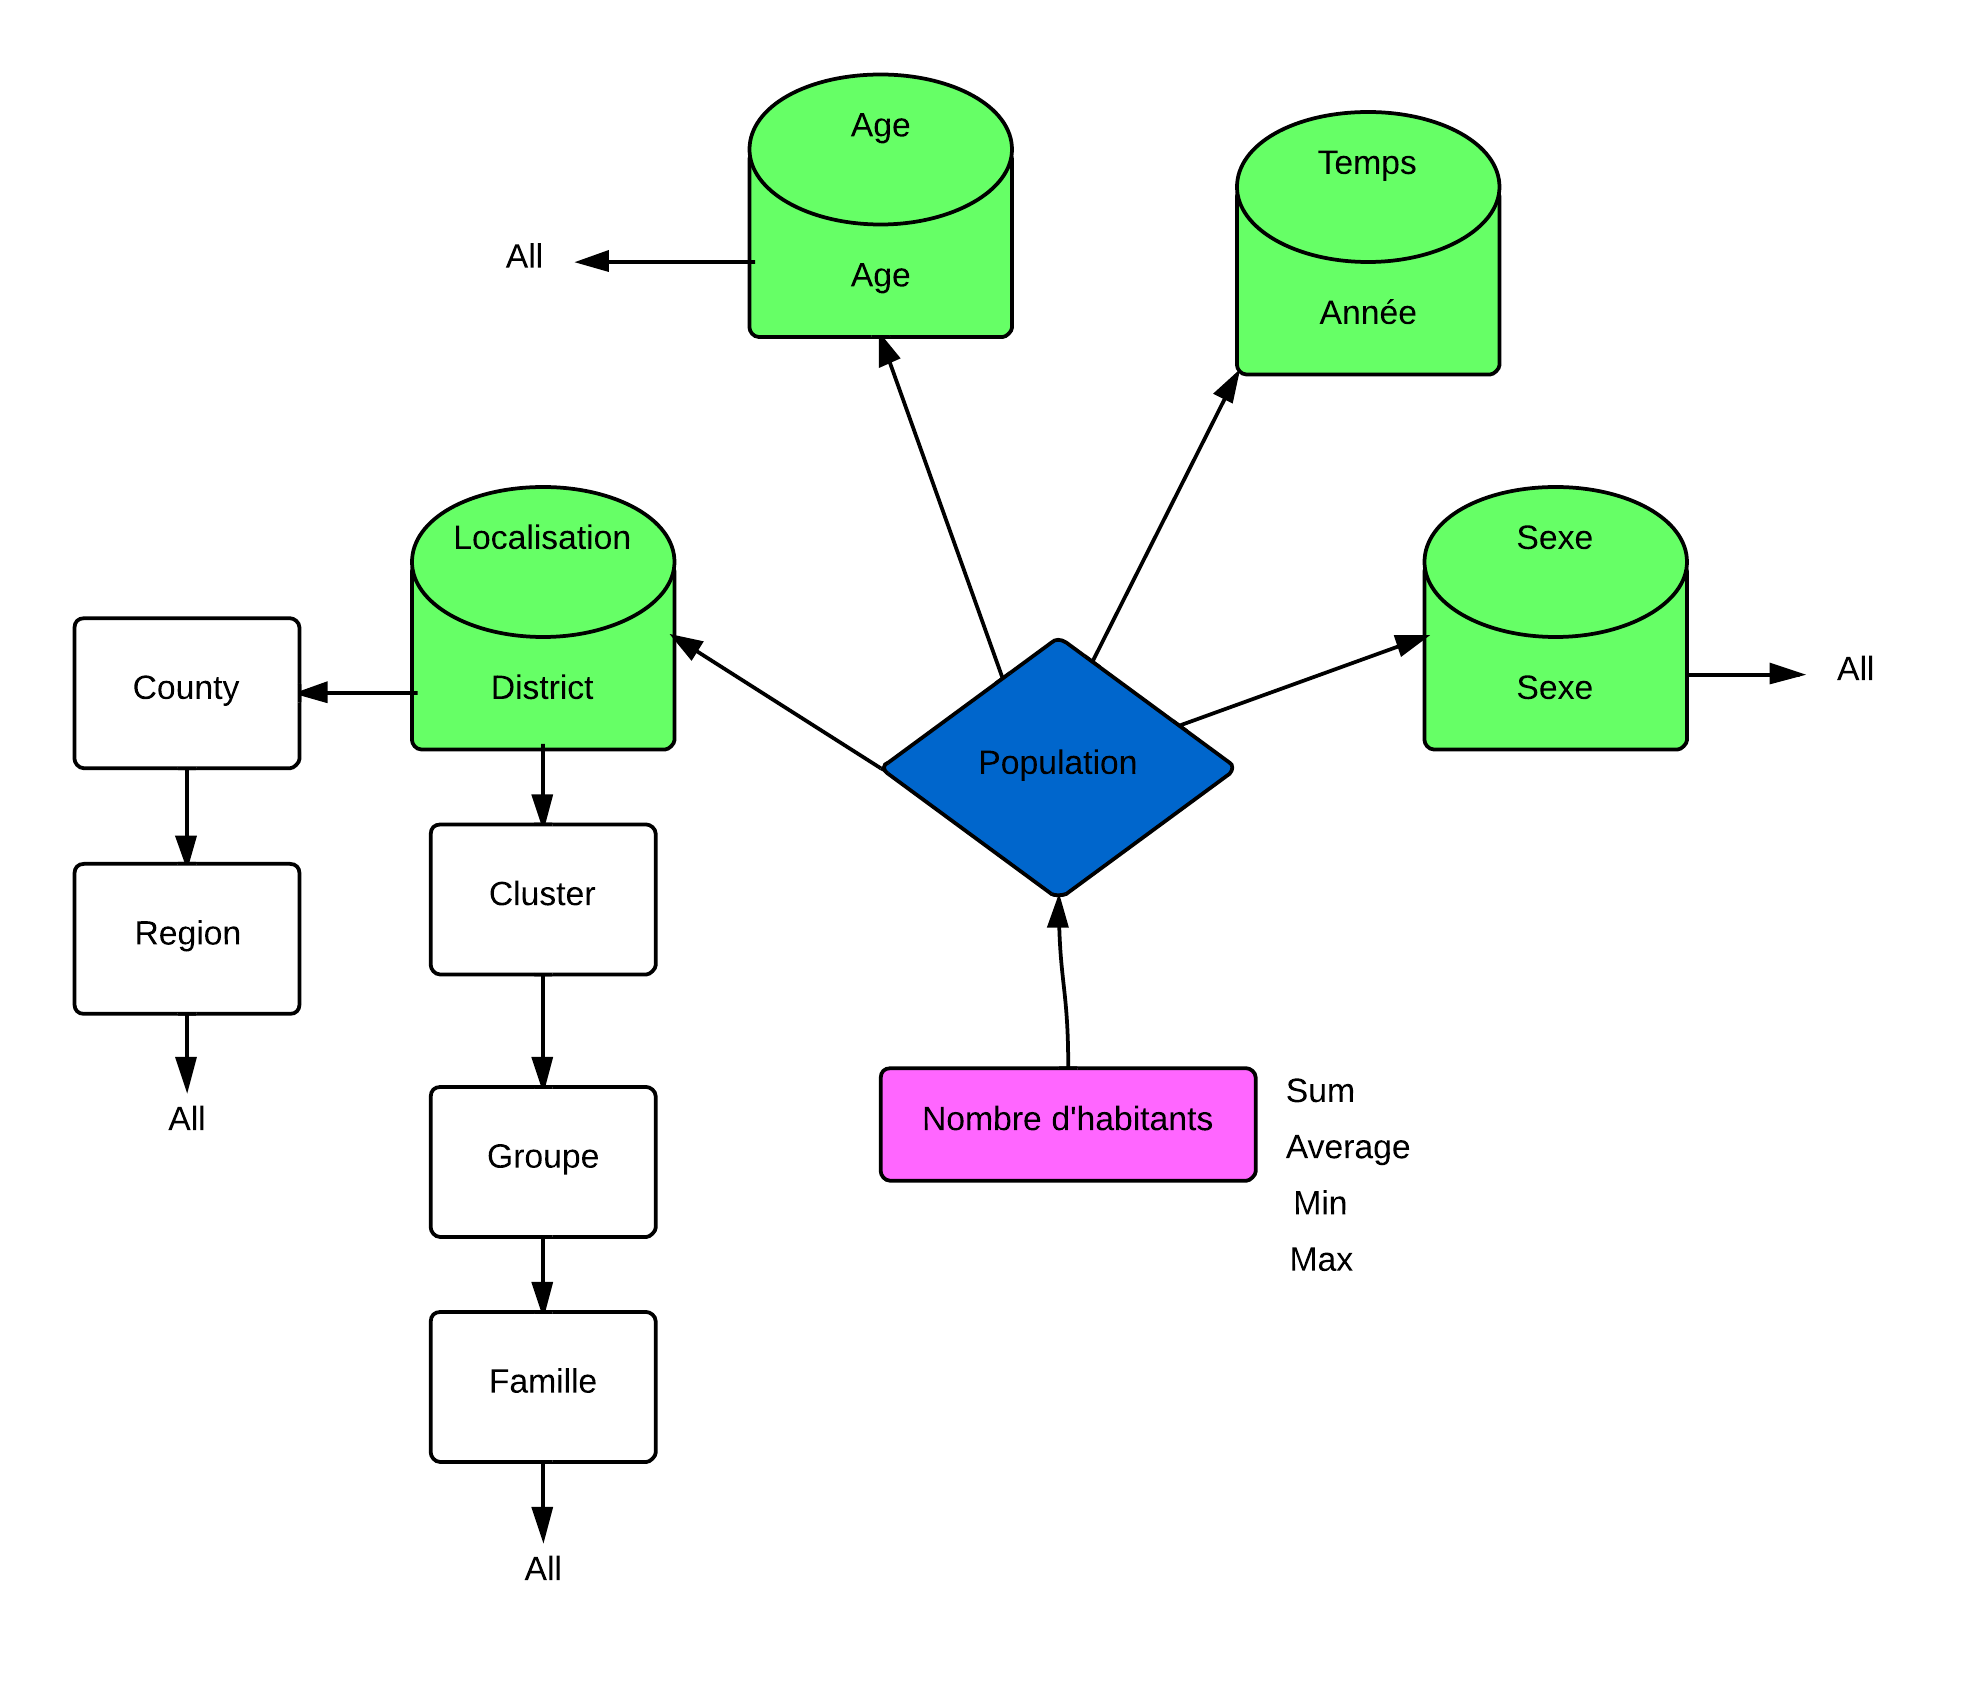
\includegraphics[width=\linewidth]{images/pop/cube.png}
    \caption{Modèle conceptuel de l'hypercube Population}
    \label{conception_cube_pop}
\end{figure}

\pagebreak

\section{Hypercube Nombre de morts}
\begin{figure}[h]
    \centering
    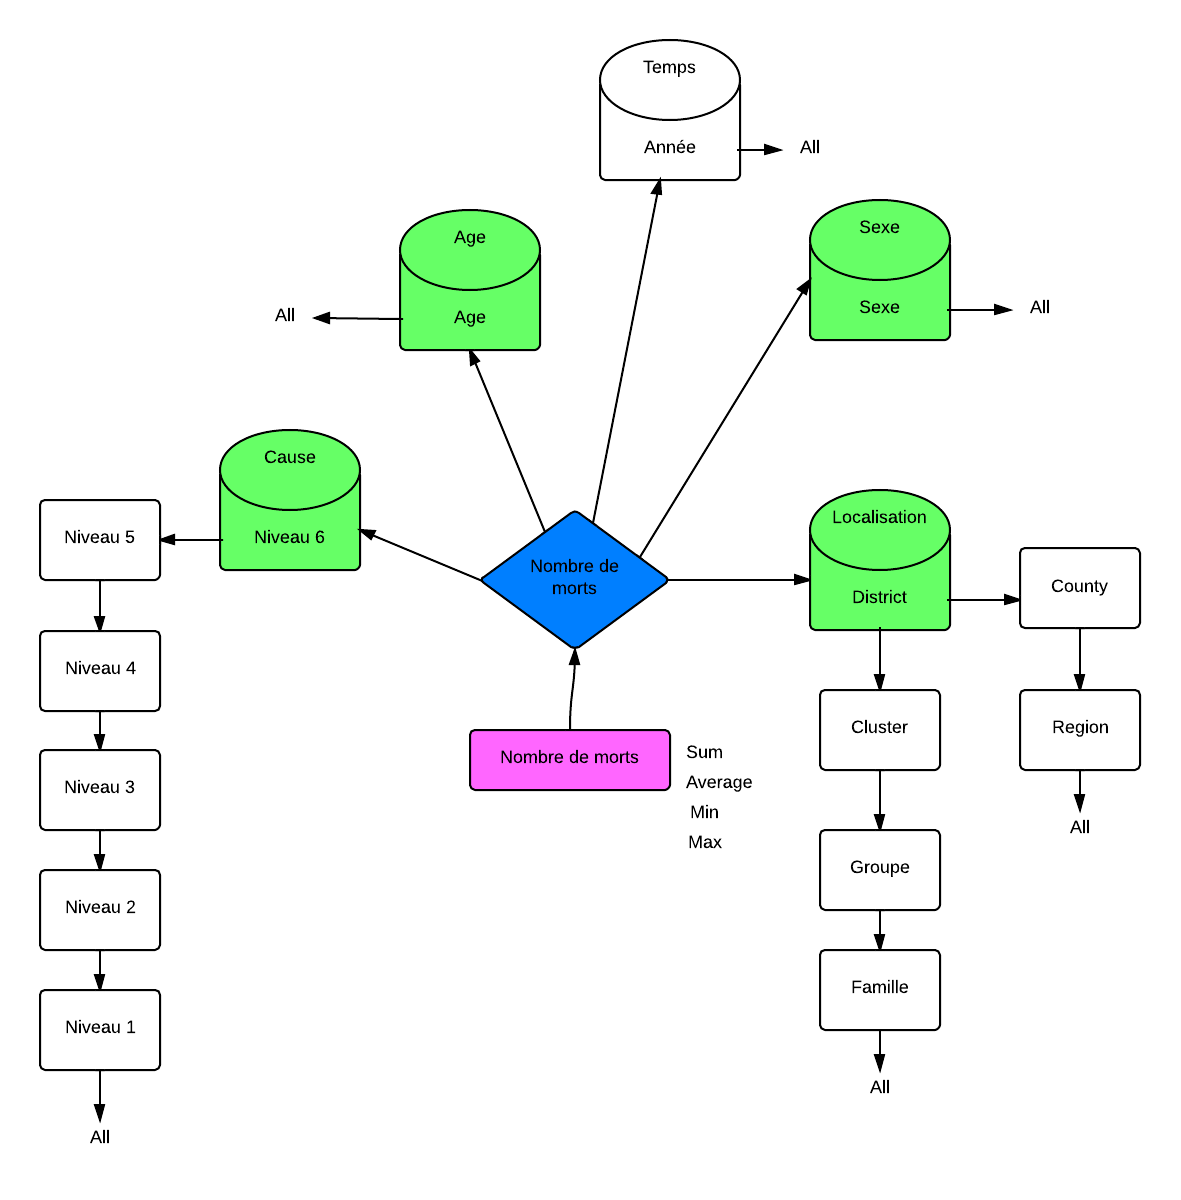
\includegraphics[width=\linewidth]{images/cubeNbMorts.png}
    \caption{Modèle conceptuel de l'hypercube Nombre de morts}
    \label{conception_cube_nombre_morts}
\end{figure}

\pagebreak

\section{Hypercube Néoplasies}
\begin{figure}[h]
    \centering
    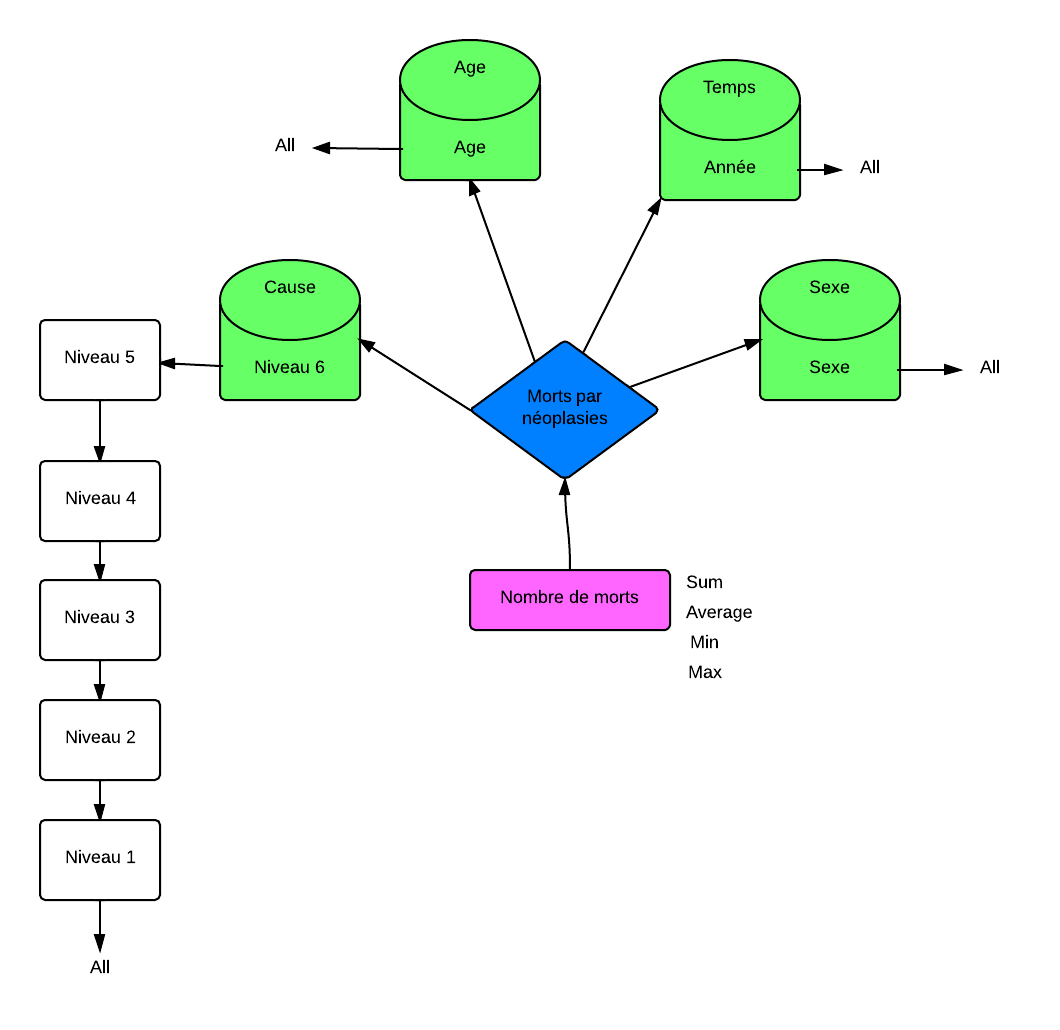
\includegraphics[width=\linewidth]{images/cubeNeo.png}
    \caption{Modèle conceptuel de l'hypercube Néoplasies}
    \label{conception_cube_néoplasies}
\end{figure}

\pagebreak

\section{Entrepôt}
\begin{figure}[h]
    \centering
    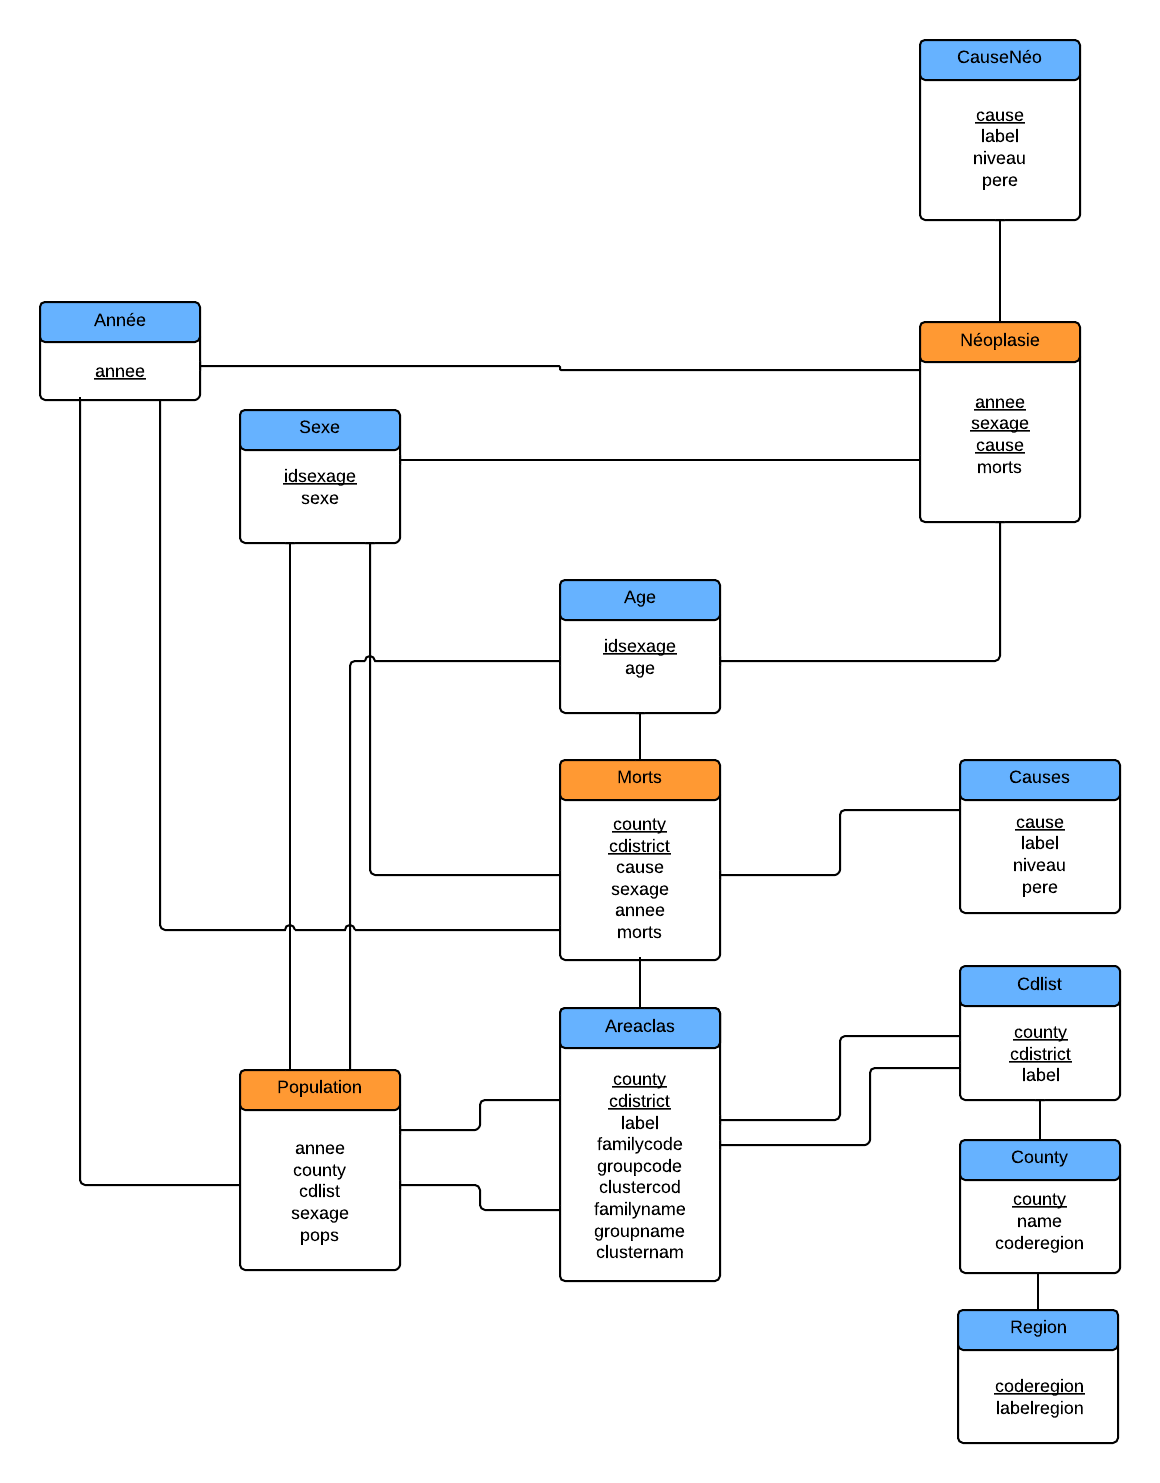
\includegraphics[width=0.8\linewidth]{images/entrepot.png}
    \caption{Modèle logique de l'entrepôt}
    \label{conception_cube_néoplasies}
\end{figure}


\chapter{Transformations des tables d'origine}

\section{Séparation des données de sexe et d'âge}

    Afin de créer deux dimensions : sexe et âge, nous avions besoin de créer deux tables. Vu le format des données de la table SexAge, dissocier l'effet du sexe et de l'âge n'était pas simple. Nous avons utilisé un requête SQL permettant de dissocier les labels M1-4, de façon à avoir une table associant l'id sexage au sexe (M ou F), et une table associant l'id sexage à la tranche d'âge (1-4).

\section{Table temporelle}

    Nous avions aussi besoin d'une dimension temps pour nos cubes, qui nécessitait une table "year". Nous avons donc simplement créer une table, avec une seule colonne, contenant les années de 79 à 92. La colonne sert à la fois d'identifiant et de données.


\section{Incohérences dans les nombres de morts}

    Comme expliquer dans l'analyse des données, les nombres de morts selon les niveaux des causes n'est pas bon. Pour l'analyse du nombre de morts, nous nous concentrons uniquement sur les causes de niveau 1 et 2. Nous souhaitions garder le "vrai" nombre de morts, c'est-à-dire les nombres obtenus pour les causes de niveau 1 (il y a moins de morts de cause de niveau 2, donc il y a eu des oublis, des erreurs de renseignement pour ces causes), tout en gardant les causes disponibles. La solution que nous avons choisi est de rajouter une nouvelle cause de mort de niveau 2 nommée "cause inconnue", afin de ne pas sous-estimer le nombre de morts en ignorant ceux dont la cause de niveau 2 n'est pas renseignée. Cette cause contiendra la différence entre la somme des morts de cause de niveau et la somme des morts de cause de niveau 2.

\section{Données des nombres de morts}

    Afin d'exploiter ces données, nous avons créé deux nouvelles tables :
    \begin{itemize}
        \item{une table "death" contenant toutes les morts de toutes les régions, uniquement pour les causes de niveau 2 (le niveau 1 étant obtenu par sommation des niveaux 2, après l'ajout de la cause inconnue), obtenue par union de toutes les tables de morts par région}
        \item{une table de cause contenant uniquement les causes de niveau 2, afin de minimiser les données}
    \end{itemize}

\section{Données des néoplasies}

    De la même façon, afin de minimiser les données, nous avons créer une nouvelle table de cause "causesNeoplasie", qui contiendra uniquement les causes concernées par les néoplasies (enfants de la cause 13). La solution la plus simple que nous avons trouvée a été de trouver dans la table de causes les lignes correspondant à ces causes. Il s'agit des lignes 13 à 44, et nous les avons simplement copiées dans notre nouvelle table "causesNeoplasie". Une autre (et meilleure) solution aurait été de parcourir récursivement les enfants de la cause 13 jusqu'à trouver tous les enfants possibles. Cette solution aurait été plus générique et plus adaptable au changement, mais il aurait fallu faire du récursif en SQL, ce qui nous paraissait très compliqué.


\pagebreak

\chapter{Indicateurs et validation}

\section{Population}
Les validations suivantes ont été appliquées sur le cube Population afin de valider l'intégrité des données de celui-ci. Les résultats obtenus lors de l'exploration du cube ont été recoupées avec les données des tables par les requêtes SQL adéquates :
\begin{itemize}
    \item Population totale en 1992 : 51 276 887. Nous avons comparé ces données à celles officielles, qui indique environ 57 millions de morts pour l'année 92. Nous avons donc le même ordre de grandeur de données.
    \item Population totale en 1992 dans le 1er county : 6 904 554
    \item Population totale en 1992, de sexe masculin et d'âge inférieur à un an : 355 930
    \item Population totale en 1992, de sexe masculin et d'âge inférieur à un an dans le 1er district et le 1er county du cluster Central London : 18
\end{itemize}


\section{Néoplasies}
Afin de valider nos données, nous avons utilisé les indicateurs suivants :
\begin{itemize}
    \item Nombre de morts de néoplasies total pour les 13 ans : 8 032 326. Il s'agit d'une simple somme de toutes les morts de la table des néoplasies. Nous avons vérifié avec les données du cube des nombres de morts, pour la région stheast et la cause 13 nous trouvons bien la même valeur.
    \item Nombre de mort d'une néoplasie de l'oesophage en 1982 : 27. Il s'agit de la somme des morts pour la cause 17 et l'année 82. Nous avons là aussi vérifier avec l'autre cube, qui trouve bien la même valeur.
    \item Moyenne du nombre de morts de néoplasies par année : 573 737,6. Là encore nous avons vérifier nos données avec l'autre cube afin d'en assurer la validité.
\end{itemize}



\pagebreak
